\documentclass[11pt,a4paper]{ctexart}
% Shared preamble for the assignment reports. Use with:
%   \documentclass[11pt,a4paper]{ctexart}  (XeLaTeX)
%   % Shared preamble for the assignment reports. Use with:
%   \documentclass[11pt,a4paper]{ctexart}  (XeLaTeX)
%   % Shared preamble for the assignment reports. Use with:
%   \documentclass[11pt,a4paper]{ctexart}  (XeLaTeX)
%   \input{../common/preamble.tex}
\usepackage[margin=2.3cm]{geometry}
\setmainfont{texgyretermes}[Extension=.otf,UprightFont=*-regular,BoldFont=*-bold,ItalicFont=*-italic,BoldItalicFont=*-bolditalic]
\setsansfont{texgyreheros}[Extension=.otf,UprightFont=*-regular,BoldFont=*-bold,ItalicFont=*-italic,BoldItalicFont=*-bolditalic]
\setmonofont{texgyrecursor}[Extension=.otf,UprightFont=*-regular,BoldFont=*-bold,ItalicFont=*-italic,BoldItalicFont=*-bolditalic]
\usepackage{amsmath,amssymb,mathtools,bm}
\usepackage{graphicx}
\usepackage{booktabs,multirow,makecell,array,tabularx}
\usepackage[table]{xcolor}
\usepackage[most]{tcolorbox}
\usepackage{enumitem}
\usepackage{listings}
\usepackage{subcaption}
\usepackage{siunitx}
\usepackage[hidelinks]{hyperref}
\usepackage[nameinlink,noabbrev]{cleveref}
\usepackage{float}

\setlength{\emergencystretch}{3em}
\linespread{1.15}
\setlist{leftmargin=*,itemsep=2pt,topsep=3pt}
\graphicspath{{figures/}}

\crefname{figure}{图}{图}
\crefname{table}{表}{表}
\crefname{section}{第}{第}
\creflabelformat{section}{#2#1#3 节}
\crefname{equation}{式}{式}
\crefformat{equation}{式~(#2#1#3)}

\lstset{basicstyle=\ttfamily\footnotesize,columns=fullflexible,breaklines=true,frame=single,
  framerule=0.3pt,rulecolor=\color{black!40},backgroundcolor=\color{black!3},
  keywordstyle=\color{blue!60!black}\bfseries,commentstyle=\color{green!40!black},
  numbers=left,numberstyle=\tiny\color{black!50},xleftmargin=1.5em}

% Interview boxes: question, model answer, common wrong answer.
\newtcolorbox{iqbox}[1]{enhanced,breakable,colback=blue!3,colframe=blue!45!black,boxrule=0.5pt,arc=1.5pt,
  left=4pt,right=4pt,top=3pt,bottom=3pt,fonttitle=\bfseries\small,title={面试追问：#1}}
\newtcolorbox{findingbox}[1][]{enhanced,breakable,colback=green!3,colframe=green!40!black,boxrule=0.5pt,arc=1.5pt,
  left=4pt,right=4pt,top=3pt,bottom=3pt,fonttitle=\bfseries\small,title={结论#1}}
\newtcolorbox{caveatbox}{enhanced,breakable,colback=orange!4,colframe=orange!60!black,boxrule=0.5pt,arc=1.5pt,
  left=4pt,right=4pt,top=3pt,bottom=3pt,fonttitle=\bfseries\small,title={不能推出的结论}}

\newcommand{\authorline}{ShaneLiu04\thanks{GitHub: \url{https://github.com/ShaneLiu04}。代码与原始指标见 edge-deploy 仓库各 lab 的 \texttt{artifacts/raw/}。本文基于公开课程材料独立完成，与课程团队无隶属关系。}}

\usepackage[margin=2.3cm]{geometry}
\setmainfont{texgyretermes}[Extension=.otf,UprightFont=*-regular,BoldFont=*-bold,ItalicFont=*-italic,BoldItalicFont=*-bolditalic]
\setsansfont{texgyreheros}[Extension=.otf,UprightFont=*-regular,BoldFont=*-bold,ItalicFont=*-italic,BoldItalicFont=*-bolditalic]
\setmonofont{texgyrecursor}[Extension=.otf,UprightFont=*-regular,BoldFont=*-bold,ItalicFont=*-italic,BoldItalicFont=*-bolditalic]
\usepackage{amsmath,amssymb,mathtools,bm}
\usepackage{graphicx}
\usepackage{booktabs,multirow,makecell,array,tabularx}
\usepackage[table]{xcolor}
\usepackage[most]{tcolorbox}
\usepackage{enumitem}
\usepackage{listings}
\usepackage{subcaption}
\usepackage{siunitx}
\usepackage[hidelinks]{hyperref}
\usepackage[nameinlink,noabbrev]{cleveref}
\usepackage{float}

\setlength{\emergencystretch}{3em}
\linespread{1.15}
\setlist{leftmargin=*,itemsep=2pt,topsep=3pt}
\graphicspath{{figures/}}

\crefname{figure}{图}{图}
\crefname{table}{表}{表}
\crefname{section}{第}{第}
\creflabelformat{section}{#2#1#3 节}
\crefname{equation}{式}{式}
\crefformat{equation}{式~(#2#1#3)}

\lstset{basicstyle=\ttfamily\footnotesize,columns=fullflexible,breaklines=true,frame=single,
  framerule=0.3pt,rulecolor=\color{black!40},backgroundcolor=\color{black!3},
  keywordstyle=\color{blue!60!black}\bfseries,commentstyle=\color{green!40!black},
  numbers=left,numberstyle=\tiny\color{black!50},xleftmargin=1.5em}

% Interview boxes: question, model answer, common wrong answer.
\newtcolorbox{iqbox}[1]{enhanced,breakable,colback=blue!3,colframe=blue!45!black,boxrule=0.5pt,arc=1.5pt,
  left=4pt,right=4pt,top=3pt,bottom=3pt,fonttitle=\bfseries\small,title={面试追问：#1}}
\newtcolorbox{findingbox}[1][]{enhanced,breakable,colback=green!3,colframe=green!40!black,boxrule=0.5pt,arc=1.5pt,
  left=4pt,right=4pt,top=3pt,bottom=3pt,fonttitle=\bfseries\small,title={结论#1}}
\newtcolorbox{caveatbox}{enhanced,breakable,colback=orange!4,colframe=orange!60!black,boxrule=0.5pt,arc=1.5pt,
  left=4pt,right=4pt,top=3pt,bottom=3pt,fonttitle=\bfseries\small,title={不能推出的结论}}

\newcommand{\authorline}{ShaneLiu04\thanks{GitHub: \url{https://github.com/ShaneLiu04}。代码与原始指标见 edge-deploy 仓库各 lab 的 \texttt{artifacts/raw/}。本文基于公开课程材料独立完成，与课程团队无隶属关系。}}

\usepackage[margin=2.3cm]{geometry}
\setmainfont{texgyretermes}[Extension=.otf,UprightFont=*-regular,BoldFont=*-bold,ItalicFont=*-italic,BoldItalicFont=*-bolditalic]
\setsansfont{texgyreheros}[Extension=.otf,UprightFont=*-regular,BoldFont=*-bold,ItalicFont=*-italic,BoldItalicFont=*-bolditalic]
\setmonofont{texgyrecursor}[Extension=.otf,UprightFont=*-regular,BoldFont=*-bold,ItalicFont=*-italic,BoldItalicFont=*-bolditalic]
\usepackage{amsmath,amssymb,mathtools,bm}
\usepackage{graphicx}
\usepackage{booktabs,multirow,makecell,array,tabularx}
\usepackage[table]{xcolor}
\usepackage[most]{tcolorbox}
\usepackage{enumitem}
\usepackage{listings}
\usepackage{subcaption}
\usepackage{siunitx}
\usepackage[hidelinks]{hyperref}
\usepackage[nameinlink,noabbrev]{cleveref}
\usepackage{float}

\setlength{\emergencystretch}{3em}
\linespread{1.15}
\setlist{leftmargin=*,itemsep=2pt,topsep=3pt}
\graphicspath{{figures/}}

\crefname{figure}{图}{图}
\crefname{table}{表}{表}
\crefname{section}{第}{第}
\creflabelformat{section}{#2#1#3 节}
\crefname{equation}{式}{式}
\crefformat{equation}{式~(#2#1#3)}

\lstset{basicstyle=\ttfamily\footnotesize,columns=fullflexible,breaklines=true,frame=single,
  framerule=0.3pt,rulecolor=\color{black!40},backgroundcolor=\color{black!3},
  keywordstyle=\color{blue!60!black}\bfseries,commentstyle=\color{green!40!black},
  numbers=left,numberstyle=\tiny\color{black!50},xleftmargin=1.5em}

% Interview boxes: question, model answer, common wrong answer.
\newtcolorbox{iqbox}[1]{enhanced,breakable,colback=blue!3,colframe=blue!45!black,boxrule=0.5pt,arc=1.5pt,
  left=4pt,right=4pt,top=3pt,bottom=3pt,fonttitle=\bfseries\small,title={面试追问：#1}}
\newtcolorbox{findingbox}[1][]{enhanced,breakable,colback=green!3,colframe=green!40!black,boxrule=0.5pt,arc=1.5pt,
  left=4pt,right=4pt,top=3pt,bottom=3pt,fonttitle=\bfseries\small,title={结论#1}}
\newtcolorbox{caveatbox}{enhanced,breakable,colback=orange!4,colframe=orange!60!black,boxrule=0.5pt,arc=1.5pt,
  left=4pt,right=4pt,top=3pt,bottom=3pt,fonttitle=\bfseries\small,title={不能推出的结论}}

\newcommand{\authorline}{ShaneLiu04\thanks{GitHub: \url{https://github.com/ShaneLiu04}。代码与原始指标见 edge-deploy 仓库各 lab 的 \texttt{artifacts/raw/}。本文基于公开课程材料独立完成，与课程团队无隶属关系。}}

\graphicspath{{../../solutions/edge-runtime/conv-kernels/artifacts/figures/}}

\title{卷积 kernel 实验报告：\\im2col、implicit GEMM、depthwise 布局与 Winograd 的速度和数值代价}
\author{\authorline}
\date{2026 年 11 月}

\begin{document}
\maketitle

\begin{abstract}
conv-kernels lab 在 9 个真实的 MobileNetV2 / ResNet 卷积层上，用单线程 fp32 C++ 实现并实测了 7 种卷积 kernel：朴素 NCHW、im2col + GEMM、
implicit GEMM、1×1 直接 GEMM、按通道的 CHW depthwise、NHWC + AVX-512 depthwise 和 Winograd F(2,3)。每种实现都和 fp64 参考逐元素比对。
另外从 Toom-Cook 插值构造了 F(2,3) / F(4,3) / F(6,3) 的变换矩阵，在 fp32 与 fp16 下测了误差。主平台是一台 4 核 Ice Lake 虚拟机（AVX-512 + VNNI），
同一份代码又在 Xeon Platinum 8470Q（Sapphire Rapids）上单线程重跑了一遍。

主要结论：
（a）implicit GEMM 与 im2col 速度相当（22.4--34.9 对 15.8--36.6 GFLOP/s），但不需要工作区；ResNet $56^2\times64$ 层的 im2col 工作区是 7.2 MB，为输入加输出的 4.5 倍；
在 IC = 3 的 stem 上，implicit GEMM 快 1.8 倍；
（b）1×1 卷积不需要 im2col：把 NHWC 输入直接当 GEMM 的 A 矩阵，两个 $56^2$ 层快 7--19\%，$14^2$ 层基本持平；
（c）depthwise 的速度由布局决定：NHWC + SIMD 跑到 10.4--11.4 GFLOP/s，按通道的 CHW 只有 1.2--1.3，相差 8.2--9.0 倍；
在同一个倒残差块里，depthwise 占 MACs 的 15.8\%，却占时间的 33.4\%（服务器上 40.1\%）；
（d）Winograd F(2,3) 在 $14^2\times256$ 层上是 implicit GEMM 的 2.15 倍（理论 2.25），在 $56^2\times64$ 层上只有 1.16 倍；
（e）数值上，fp16 下 F(2,3) 与直接卷积精度相同（2.2e-3 对 2.0e-3），F(4,3) 的误差是直接卷积的 7.2 倍，插值点换成 0..4 就直接溢出；
int8 输入经 F(2,3) 变换后需要 10 bit，经 F(4,3) 变换后需要 15 bit；
（f）换到 Xeon 8470Q 后，GEMM 类卷积快 2.0--2.8 倍（$14^2$ ResNet 层除外），Winograd 在 $56^2$ 层上只快 1.37 倍，于是从“快 16\%”翻转成“慢 32\%”；
depthwise 的 NHWC 优势（8.2 倍）不随机器变化。
\end{abstract}

\tableofcontents
\newpage

\section{这个实验要回答什么}\label{sec:questions}

卷积是端侧视觉模型里耗时最多的算子。工程上常见的实现有三类：把每个输出位置的感受野展开成矩阵一行再调 GEMM 的 im2col~\cite{chellapilla2006}；
不展开、在 GEMM 的取数地址里直接按卷积下标计算的 implicit GEMM；在变换域里用更少乘法算一个输出 tile 的 Winograd~\cite{lavin2016}。
depthwise 卷积不跨通道求和，GEMM 化没有意义，要单独写 kernel。MIT 6.5940 的 TinyEngine~\cite{mcunet} 一讲讨论了 im2col 的内存代价与 depthwise 的原地计算，
CMU 15-418 讲了分块与 SIMD。这个 lab 把这些说法放到同一组层、同一台机器上实测，回答五个问题：

\begin{enumerate}
  \item \textbf{im2col 的工作区值不值}：展开后 GEMM 更规整，但工作区与输入、输出同时存活。implicit GEMM 去掉工作区后会不会变慢？（\cref{sec:res-gemm}）
  \item \textbf{1×1 卷积与 stem 是否例外}：1×1 时 NHWC 输入本身就是 im2col 矩阵；stem 的 K 维只有 27。这两类层上谁快？（\cref{sec:res-pw,sec:res-stem}）
  \item \textbf{depthwise 靠什么提速}：算术强度很低、没有跨通道归约，布局能带来多少差别？它在一个倒残差块里占多少时间？（\cref{sec:res-dw}）
  \item \textbf{Winograd 的实测加速离理论多远}：F(2,3) 理论上少 2.25 倍乘法，两个 MACs 相同的 ResNet~\cite{resnet} 层上实测分别是多少，差别从哪里来？（\cref{sec:res-wino}）
  \item \textbf{Winograd 的数值代价}：tile 变大、插值点变化时，fp32 / fp16 误差如何增长？int8 能不能用？（\cref{sec:numerics}）
\end{enumerate}

最后，同一份代码在 Xeon 8470Q 上重跑，用来区分“结构性”结论（由访存 / 计算比决定，换机器只改变常数）和“位置性”结论（取决于两个量的相对大小，换机器可能翻转），
见 \cref{sec:cross}。跨平台的整体讨论在 edge-runtime-server 报告里；本报告是这个 lab 的专门分析，可以独立阅读。

\section{设置}\label{sec:setup}

\subsection{平台}

\begin{table}[H]
\centering\small
\caption{平台与协议}\label{tab:setup}
\begin{tabularx}{\linewidth}{>{\raggedright\arraybackslash}p{1.7cm} >{\raggedright\arraybackslash}X >{\raggedright\arraybackslash}X}
\toprule
 & 本机（主平台） & 服务器复现 \\
\midrule
CPU & Ice Lake 服务器 CPU 的 Windows Server 虚拟机，4 物理核 / 8 逻辑核（Family 6 Model 106） & 2 × Xeon Platinum 8470Q（Sapphire Rapids），绑 NUMA1 物理核 \\
ISA & AVX-512F、AVX-512 VNNI、AVX2、FMA & 同左，另有 AMX-INT8（本 lab 的 fp32 kernel 不使用） \\
编译器 & MinGW g++ 13.2，\texttt{-O3 -std=c++17 -march=native -fno-math-errno} & GCC 11.4，同样的选项 \\
屋顶（1 线程） & fp32 154.9 GFLOP/s，DRAM 只读 13.4 GB/s，L2 1.25 MiB/核（host-roofline） & fp32 232 GFLOP/s，DRAM 只读 17.5 GB/s（host-roofline） \\
线程 & 1 & 1 \\
原始数据 & \nolinkurl{artifacts/raw/} & \nolinkurl{artifacts/raw/xeon8470q/} \\
\bottomrule
\end{tabularx}
\end{table}

\paragraph{计时。} 每个 kernel 先预热 2 次；单次调用若短于 20 ms，就在一个样本里循环多次再取平均，使每个样本至少 20 ms；共 15 个样本，报告中位数（p50），
CSV 里同时保留 p10、p90 与最小值。本机所有点的 p90/p50 不超过 1.42（出现在 depthwise $14^2$ 的朴素实现上），服务器上不超过 1.13。
GFLOP/s 按 $2\times\text{MACs}/t_{p50}$ 计；Winograd 也按直接卷积的 MACs 计，所以它的数字是\emph{等效} GFLOP/s，可以直接与其他实现比较时间。

\paragraph{正确性。} 参考实现是 fp64、NCHW 布局、OIHW 权重；被测 kernel 用 NHWC 激活和 \texttt{[KH][KW][IC][OC]}（dense）或 \texttt{[KH][KW][C]}（depthwise）权重，
所以比对同时检查了布局转换。误差定义为 $\max|y-y_\text{ref}| / \max|y_\text{ref}|$。\texttt{--mode=check} 在 7 个小形状（含 stride 2、5×5、奇数尺寸的部分 tile）上检查全部实现，
\texttt{--mode=bench} 在 9 个真实层上计时的同时再比对一次。

\subsection{9 个层}

\begin{table}[H]
\centering\small
\caption{被测层（MACs 与激活字节取自 \texttt{conv\_bench.csv}；激活字节 = fp32 输入 + 输出）}\label{tab:layers}
\resizebox{\linewidth}{!}{\begin{tabular}{llllrrr}
\toprule
层 & 输入 & 通道 & 核 / 步长 & MACs & 激活字节 & im2col 工作区 \\
\midrule
\texttt{mbv2\_stem\_224} & $224^2$ & 3 → 32 & 3×3 / 2 & 10,838,016 & 2,207,744 & 1,354,752 \\
\texttt{mbv2\_pw\_expand\_56} & $56^2$ & 24 → 144 & 1×1 / 1 & 10,838,016 & 2,107,392 & 301,056 \\
\texttt{mbv2\_dw\_56} & $56^2$ & 144（dw） & 3×3 / 1 & 4,064,256 & 3,612,672 & -- \\
\texttt{mbv2\_pw\_project\_56} & $56^2$ & 144 → 24 & 1×1 / 1 & 10,838,016 & 2,107,392 & 1,806,336 \\
\texttt{mbv2\_dw\_s2\_56} & $56^2$ & 144（dw） & 3×3 / 2 & 1,016,064 & 2,257,920 & -- \\
\texttt{mbv2\_dw\_14} & $14^2$ & 576（dw） & 3×3 / 1 & 1,016,064 & 903,168 & -- \\
\texttt{mbv2\_pw\_expand\_14} & $14^2$ & 96 → 576 & 1×1 / 1 & 10,838,016 & 526,848 & 75,264 \\
\texttt{resnet\_3x3\_56} & $56^2$ & 64 → 64 & 3×3 / 1 & 115,605,504 & 1,605,632 & 7,225,344 \\
\texttt{resnet\_3x3\_14} & $14^2$ & 256 → 256 & 3×3 / 1 & 115,605,504 & 401,408 & 1,806,336 \\
\bottomrule
\end{tabular}}
\end{table}

前 7 层来自 MobileNetV2~\cite{mobilenetv2}：stem、一个 $56^2$ 的倒残差块（expand、depthwise、project）、stride 2 的 depthwise，以及 $14^2$ 的一对 depthwise / expand。
两个 ResNet 层的 MACs 完全相同（1.16 亿），只是“空间大、通道少”与“空间小、通道多”的区别，正好用来隔离通道数对 Winograd 的影响。

\subsection{7 种实现}

\begin{table}[H]
\centering\small
\caption{\texttt{cpp/conv.cpp} 中的实现}\label{tab:impls}
\begin{tabularx}{\linewidth}{>{\raggedright\arraybackslash}p{3.0cm} >{\raggedright\arraybackslash}p{1.6cm} >{\raggedright\arraybackslash}X}
\toprule
实现 & 适用层 & 要点 \\
\midrule
\texttt{naive\_nchw} & 全部 & 六重循环、标量、NCHW，每个 tap 判断越界 \\
\texttt{im2col\_gemm} & dense & 展开到 $(OH\cdot OW)\times(K^2\cdot IC)$ 工作区，再调 6 行 × 32 列寄存器块的 AVX-512 GEMM \\
\texttt{implicit\_gemm} & dense & 不展开；4 个输出像素 × 32 个输出通道的寄存器块，取数时按 $(k_h,k_w,ic)$ 算地址，越界 tap 读一行全零 \\
\texttt{pointwise\_gemm} & 1×1，s1 & NHWC 输入就是 $(H\cdot W)\times IC$ 矩阵，直接调同一个 GEMM \\
\texttt{dw\_generic\_chw} & depthwise & 没有专用 depthwise kernel 的框架会做的事：逐通道、CHW、标量 \\
\texttt{dw\_nhwc\_simd} & depthwise & NHWC，每个 tap 一次连续加载 16 个通道，9 次 FMA 累加 \\
\texttt{winograd\_f2x3} & 3×3，s1 & 权重变换一次；输入变换 → 16 个独立 GEMM → 输出变换 \\
\bottomrule
\end{tabularx}
\end{table}

教学用的 GEMM 没有做 B 矩阵打包，寄存器块也只是 6×32（不是生产库调过的形状），所以 GEMM 类卷积只到本机 fp32 峰值的 10--24\%。
这不影响本报告的比较：im2col、implicit GEMM、pointwise 和 Winograd 的逐点乘共享同一套微核思路，差别只在取数方式与工作区。

\section{方法与推导}\label{sec:method}

\subsection{im2col 与它的工作区（E19）}

设输入 $H\times W\times IC$（NHWC），卷积核 $K_H\times K_W$，输出 $OH\times OW\times OC$。im2col 把输出位置 $(o_y,o_x)$ 的感受野
$\{x[o_y s+k_y-p,\,o_x s+k_x-p,\,ic]\}$ 拼成一行，所有输出位置构成矩阵 $\mathbf{A}\in\mathbb{R}^{(OH\cdot OW)\times(K_HK_W\cdot IC)}$，
与权重 $\mathbf{W}\in\mathbb{R}^{(K_HK_W\cdot IC)\times OC}$ 相乘就是卷积。工作区大小（公式卡 E19）为
\begin{equation}
  W_\text{im2col} = OH\cdot OW\cdot K_H\cdot K_W\cdot IC\cdot b,\label{eq:im2col}
\end{equation}
$b$ 是元素字节数。stride 1 时每个输入元素被复制 $K_HK_W$ 次，所以工作区约是输入的 $K_HK_W$ 倍。代入 ResNet $56^2\times64$、3×3、fp32：
\[
  W = 56\cdot56\cdot9\cdot64\cdot4 = 7{,}225{,}344\ \text{B},\qquad
  \frac{W}{\text{输入}+\text{输出}} = \frac{7{,}225{,}344}{1{,}605{,}632} = 4.5,
\]
与实测的 \texttt{workspace\_bytes} 一致。$14^2\times256$ 层同样是 4.5 倍（1,806,336 B）；stem 是 $112\cdot112\cdot27\cdot4 = 1{,}354{,}752$ B。
这块内存与输入、输出同时存活，必须计入静态内存规划的 arena；在只有几百 KB SRAM 的 MCU 上，它往往比权重先撞上限。CMSIS-NN 的 partial im2col 一次只展开 2 个输出位置，
把工作区降到 $2K_HK_W\cdot IC\cdot b$。

\subsection{implicit GEMM}

implicit GEMM 把 GEMM 的 K 维（长度 $K_HK_W\cdot IC$）直接映射回 $(k_y,k_x,ic)$，在加载 A 矩阵元素时计算输入地址，越界就当 padding。
本 lab 的实现（\cref{lst:implicit}）把 4 个输出像素的源指针在 $(k_h,k_w)$ 循环里算好，越界的 tap 指向一行全零，于是最内层的 $ic$ 循环没有分支，
每步 2 次 512 位权重加载、4 次广播、8 次 FMA。它和 im2col 做的算术完全相同，连累加顺序都一样（K 维按 $k_h,k_w,ic$ 遍历），
所以 \texttt{cpp\_check.csv} 里两者在每个形状上的误差逐位相同（例如本机 \texttt{dense5x5} 都是 2.75e-7）。

\begin{lstlisting}[language=C++,caption={implicit GEMM 的内层（节选自 \texttt{conv\_implicit}）},label={lst:implicit}]
for (int kh = 0; kh < L.k; ++kh)
  for (int kw = 0; kw < L.k; ++kw) {
    const float* src[4];
    for (int r = 0; r < 4; ++r) {
      int ih = ohs[r] * L.stride + kh - pad, iw = ows[r] * L.stride + kw - pad;
      src[r] = (ih < 0 || ih >= L.h || iw < 0 || iw >= L.w) ? zero_row.data()
               : x + (static_cast<size_t>(ih) * L.w + iw) * L.ic;
    }
    const float* wk = w + static_cast<size_t>((kh * L.k + kw) * L.ic) * N;
    for (int ic = 0; ic < L.ic; ++ic) {
      __m512 b0 = _mm512_maskz_loadu_ps(m0, wk + static_cast<size_t>(ic) * N + j);
      __m512 b1 = _mm512_maskz_loadu_ps(m1, wk + static_cast<size_t>(ic) * N + j + 16);
      for (int r = 0; r < 4; ++r) {
        __m512 a = _mm512_set1_ps(src[r][ic]);
        c[r][0] = _mm512_fmadd_ps(a, b0, c[r][0]);
        c[r][1] = _mm512_fmadd_ps(a, b1, c[r][1]);
      }
    }
  }
\end{lstlisting}

代价是 A 的地址不再连续：每 $IC$ 个元素换一次源指针。$IC$ 越小，换指针越频繁；但 im2col 在同样的地方要做一次 \texttt{memcpy}，
所以小 $IC$ 时 im2col 的代价更大（\cref{sec:res-stem}）。

\paragraph{1×1 卷积。} 1×1、stride 1 时感受野只有一个像素的 $IC$ 个通道，NHWC 下输入本身就是 $(H\cdot W)\times IC$ 的矩阵，
\cref{eq:im2col} 退化为一次 $H\cdot W\cdot IC\cdot b$ 的拷贝。\texttt{pointwise\_gemm} 直接把输入当 A 矩阵，连这次拷贝也省掉。

\subsection{depthwise：强度与布局（E21）}

depthwise 卷积每个输出通道只依赖同一个输入通道，没有跨通道求和，等价 GEMM 的 K 维只有 $K_HK_W = 9$，寄存器分块无从谈起。
若每个输入元素只从内存读一次，算术强度（公式卡 E21）为
\begin{equation}
  I_\text{dw} = \frac{2K_HK_W}{b}\ \text{FLOP/B}, \qquad \text{fp32 3×3：} I = 4.5,\label{eq:dw}
\end{equation}
远在本机 fp32 拐点 $154.9/13.4 = 11.5$ FLOP/B 的左边。按“输入、输出各读写一次”计入输出字节时，$56^2\times144$ 层是 $8.1\ \text{MFLOP} / 3.6\ \text{MB} \approx 2.25$ FLOP/B，
从 DRAM 供数的上限约 $2.25\times13.4\approx30$ GFLOP/s；stride 2 的层输出少 4 倍、FLOP 也少 4 倍，强度只有 0.9 FLOP/B。

布局决定能不能向量化。CHW 下按通道循环，SIMD 只能沿空间维展开，3×3 窗口的边界判断落在每个 tap 上；NHWC 下通道维连续，
\texttt{dw\_nhwc\_simd} 对每个输出像素按 16 个通道一组做 9 次“加载输入 + 加载权重 + FMA”，边界判断与通道无关，只在 $(k_h,k_w)$ 层做一次。
$C = 144$ 恰好是 9 个向量，$C = 576$ 是 36 个，都没有尾部掩码。

\subsection{Winograd：Toom-Cook 构造（E20）}\label{sec:toomcook}

\paragraph{1-D 情形。} $r$ 抽头相关 $y_i = \sum_{k=0}^{r-1} g_k d_{i+k}$（$i = 0,\dots,m-1$）直接计算要 $mr$ 次乘法。
它是多项式乘法的转置：两个次数为 $m-1$ 与 $r-1$ 的多项式之积有 $n = m+r-1$ 个系数，可以在 $n$ 个点上求值、逐点相乘、再插值回来，只用 $n$ 次乘法。
\texttt{code/convlab/winograd.py} 取 $n-1$ 个有限点 $a_0,\dots,a_{n-2}$ 加上无穷远点，按下式精确地（有理数）构造三个矩阵：
\begin{align}
  G_{jk} &= \frac{a_j^k}{f_j},\quad f_j = \prod_{l\neq j}(a_j-a_l), & G_{\infty} &= e_{r-1}^{\mathsf T}, \notag\\
  A_{ji} &= a_j^i, & A_{\infty} &= e_{m-1}^{\mathsf T}, \label{eq:toomcook}\\
  B_{:,j} &= \text{coef}\Big(\prod_{l\neq j}(x-a_l)\Big), & B_{:,\infty} &= \text{coef}\Big(\prod_{l}(x-a_l)\Big), \notag
\end{align}
于是 $y = A^{\mathsf T}\big[(Gg)\odot(B^{\mathsf T}d)\big]$。2-D 情形把两个 1-D 变换嵌套：
\begin{equation}
  Y = A^{\mathsf T}\Big[\big(G\,g\,G^{\mathsf T}\big)\odot\big(B^{\mathsf T} d\,B\big)\Big]A,\label{eq:wino2d}
\end{equation}
每个 $m\times m$ 输出 tile 的乘法从 $m^2r^2$ 降到 $n^2 = (m+r-1)^2$（公式卡 E20）：
\begin{equation}
  \text{乘法减少} = \frac{m^2r^2}{(m+r-1)^2}:\quad \text{F(2,3)}\ \tfrac{36}{16}=2.25,\quad \text{F(4,3)}\ \tfrac{144}{36}=4,\quad \text{F(6,3)}\ \tfrac{324}{64}=5.06.\label{eq:reduction}
\end{equation}

\paragraph{F(2,3) 的矩阵。} 取点 $\{0,1,-1,\infty\}$，代码生成（\texttt{transform(2)} 的输出）：
\[
B^{\mathsf T} = \begin{bmatrix} -1 & 0 & 1 & 0\\ 0 & 1 & 1 & 0\\ 0 & -1 & 1 & 0\\ 0 & -1 & 0 & 1\end{bmatrix},\quad
G = \begin{bmatrix} -1 & 0 & 0\\ \tfrac12 & \tfrac12 & \tfrac12\\ \tfrac12 & -\tfrac12 & \tfrac12\\ 0 & 0 & 1\end{bmatrix},\quad
A^{\mathsf T} = \begin{bmatrix} 1 & 1 & 1 & 0\\ 0 & 1 & -1 & 1\end{bmatrix}.
\]
例如 $f_0 = (0-1)(0+1) = -1$，所以 $G$ 第一行是 $[1,0,0]/(-1)$；$B$ 第一列是 $(x-1)(x+1) = x^2-1$ 的系数 $[-1,0,1,0]$。
与 Lavin \& Gray 的矩阵相比，$B^{\mathsf T}$ 与 $G$ 的第一行同时变号，逐点乘后抵消；\texttt{test\_f23\_matches\_lavin\_matrices} 按绝对值检查了这一点。
$B^{\mathsf T}$ 与 $A^{\mathsf T}$ 只有 $0,\pm1$，变换只需加减。

\paragraph{F(4,3) 的矩阵。} 取点 $\{0,\pm1,\pm2,\infty\}$：
\[
B^{\mathsf T} = \begin{bmatrix} 4 & 0 & -5 & 0 & 1 & 0\\ 0 & -4 & -4 & 1 & 1 & 0\\ 0 & 4 & -4 & -1 & 1 & 0\\ 0 & -2 & -1 & 2 & 1 & 0\\ 0 & 2 & -1 & -2 & 1 & 0\\ 0 & 4 & 0 & -5 & 0 & 1\end{bmatrix},\quad
A^{\mathsf T} = \begin{bmatrix} 1 & 1 & 1 & 1 & 1 & 0\\ 0 & 1 & -1 & 2 & -2 & 0\\ 0 & 1 & 1 & 4 & 4 & 0\\ 0 & 1 & -1 & 8 & -8 & 1\end{bmatrix}.
\]
$B^{\mathsf T}$ 的系数已到 5，$A^{\mathsf T}$ 到 8；$G$ 的元素是 $1/4,\ 1/6,\ 1/12,\ 1/24$ 这样的分数，在二进制里不能精确表示。

\paragraph{多通道与工作区。} 多通道时在变换域对 $IC$ 求和：$M_e = \sum_{ic} U_e[ic,oc]\,V_e[t,ic]$，$e$ 遍历 $n^2$ 个变换域位置，
于是逐点乘变成 $n^2$ 个独立的 GEMM，形状为 $(\text{tile 数})\times OC\times IC$。F(2,3) 的实现分配三块缓冲（\texttt{wino\_plan}）：
$U$ = $16\cdot IC\cdot OC\cdot4$ B（变换后的权重），$V$ = $16\cdot T\cdot IC\cdot4$ B，$M$ = $16\cdot T\cdot OC\cdot4$ B，$T$ 为 tile 数。

\begin{table}[H]
\centering\small
\caption{Winograd F(2,3) 的工作区组成（按代码公式计算，总和与 \texttt{workspace\_bytes} 一致）}\label{tab:winows}
\begin{tabular}{lrrrrr}
\toprule
层 & tile 数 $T$ & $U$ & $V$ & $M$ & 合计 \\
\midrule
$56^2\times64$ & 784 & 262,144 & 3,211,264 & 3,211,264 & 6,684,672 \\
$14^2\times256$ & 49 & 4,194,304 & 802,816 & 802,816 & 5,799,936 \\
\bottomrule
\end{tabular}
\end{table}

$56^2$ 层的大头是逐 tile 的 $V$、$M$（各 3.2 MB），$14^2$ 层的大头是变换后的权重 $U$（4.2 MB，部署时离线算好、常驻）。
两者都超过本机每核 1.25 MiB 的 L2。

\paragraph{变换开销与通道数。} 按 \texttt{conv\_winograd} 的写法数运算：每个 tile、每个输入通道的输入变换是 32 次加减，每个输出通道的输出变换是 24 次，
逐点乘 GEMM 是 $16\cdot IC\cdot OC$ 次 FMA。于是变换与 GEMM 的运算量之比为
\begin{equation}
  \frac{32\,IC + 24\,OC}{2\cdot16\cdot IC\cdot OC} \approx \frac{2}{C}\quad(IC = OC = C),\label{eq:txratio}
\end{equation}
$C = 64$ 时是 2.7\%，$C = 256$ 时是 0.68\%，相差 4 倍。按运算量看变换微不足道；但它是逐通道的标量循环（代码里没有手写 SIMD），
每个 tile 要从 16 个分散位置取数、向 16 个缓冲散布写，时间上的占比远高于运算量占比（\cref{sec:res-wino} 给出估计）。

\subsection{Winograd 的数值：为什么误差随 tile 增长}\label{sec:numerics-theory}

\cref{eq:toomcook} 里，$B$ 的列是以其余点为根的多项式的系数，点越多、越大，系数按根的绝对值的乘积增长；$G$ 的分母 $f_j$ 也随之增大。
变换后的动态范围由 $B^{\mathsf T}$ 行的 $L_1$ 范数决定，2-D 时平方：
\begin{equation}
  \text{输入放大} = \frac{\max|B^{\mathsf T}dB|}{\max|d|} \le \Big(\max_i \sum_j |B^{\mathsf T}_{ij}|\Big)^2 = \|B^{\mathsf T}\|_\infty^2.\label{eq:growth}
\end{equation}

\begin{table}[H]
\centering\small
\caption{各变体的乘法减少与范数（\texttt{transform()} 计算；$\|B^{\mathsf T}\|_\infty$ 为最大行 $L_1$ 范数）}\label{tab:norms}
\begin{tabular}{lrrrr}
\toprule
变体 & 乘法减少 & $\|B^{\mathsf T}\|_\infty$ & 输入放大 & $\max|A^{\mathsf T}_{ij}|$ \\
\midrule
F(2,3)，点 $\{0,\pm1\}$ & 2.25 & 2 & 4 & 1 \\
F(4,3)，点 $\{0,\pm1,\pm2\}$ & 4 & 10 & 100 & 8 \\
F(6,3)，点 $\{0,\pm1,\pm2,\pm\tfrac12\}$ & 5.06 & 15 & 225 & 32 \\
F(4,3)，点 $\{0,1,2,3,4\}$ & 4 & 120 & 14,400 & 64 \\
F(6,3)，点 $\{0,\pm1,\pm2,\pm3\}$ & 5.06 & 100 & 10,000 & 243 \\
\bottomrule
\end{tabular}
\end{table}

放大 100 倍约吃掉 $\log_2 100\approx6.6$ bit 的余量。fp32 有 24 位尾数，仍然够用；fp16 只有 11 位，就只剩一半。fp16 的最大值是 65,504，
放大 14,400 倍时输入只要超过约 4.5 就会溢出。int8 输入 $|d|\le127$ 经 F(2,3) 变换后最大 $4\times127 = 508$，有符号要 10 bit；
F(4,3) 最大 $100\times127 = 12{,}700$，要 15 bit。点集的选择不是自由的：$\{0,\pm1,\pm2,\pm\tfrac12\}$ 是经验上范数最小的一族，
cuDNN 提供 F(4,3)，NNPACK 的 \texttt{wt8x8} 就是这里的 F(6,3)。

\section{结果：9 层 × 7 种实现}\label{sec:results}

\begin{figure}[H]
\centering
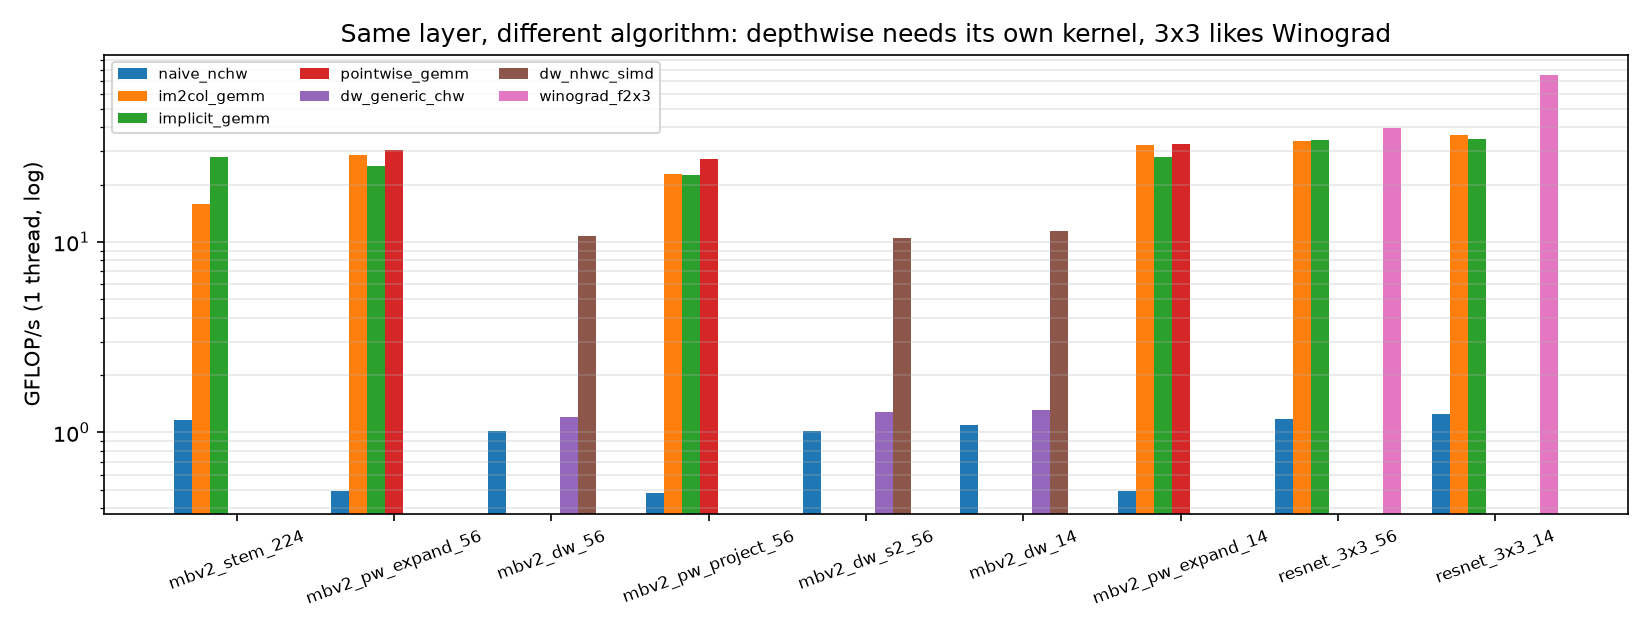
\includegraphics[width=\linewidth]{conv_bench.png}
\caption{本机（Ice Lake VM）单线程 fp32 的 GFLOP/s，对数纵轴。每组柱子是同一层上的各个实现；Winograd 按直接卷积的 FLOP 计等效值。}\label{fig:bench}
\end{figure}

\Cref{fig:bench} 的纵轴是对数，可以一眼看出三层结构：所有朴素 NCHW 实现（蓝色）挤在 0.5--1.3 GFLOP/s；depthwise 的两个实现之间隔着一个数量级
（紫色 CHW 约 1.2--1.3、棕色 NHWC 约 10--11）；GEMM 类实现（橙、绿、红）在 15--37 GFLOP/s 一带。最右边粉色的 Winograd 在 $14^2$ 层上明显高出一截（75.0），
在 $56^2$ 层上只比旁边的 GEMM 柱子高一点（39.7）。标题里的两句话就是本节要展开的结论：depthwise 需要自己的 kernel，3×3 偏爱 Winograd——后一句只在本机成立，
\cref{sec:cross} 会看到它在服务器上翻转。

\begin{table}[H]
\centering\small
\caption{本机全部结果（GFLOP/s，\texttt{conv\_bench.csv} 的 p50）}\label{tab:local}
\resizebox{\linewidth}{!}{\begin{tabular}{lrrrrrrr}
\toprule
层 & naive NCHW & im2col & implicit & pointwise & dw CHW & dw NHWC & Winograd \\
\midrule
\texttt{mbv2\_stem\_224} & 1.16 & 15.8 & \textbf{27.8} & & & & \\
\texttt{mbv2\_pw\_expand\_56} & 0.49 & 28.5 & 25.0 & \textbf{30.5} & & & \\
\texttt{mbv2\_dw\_56} & 1.02 & & & & 1.20 & \textbf{10.8} & \\
\texttt{mbv2\_pw\_project\_56} & 0.48 & 22.8 & 22.4 & \textbf{27.2} & & & \\
\texttt{mbv2\_dw\_s2\_56} & 1.02 & & & & 1.28 & \textbf{10.4} & \\
\texttt{mbv2\_dw\_14} & 1.10 & & & & 1.32 & \textbf{11.4} & \\
\texttt{mbv2\_pw\_expand\_14} & 0.49 & 32.4 & 28.1 & \textbf{32.9} & & & \\
\texttt{resnet\_3x3\_56} & 1.18 & 33.9 & 34.3 & & & & \textbf{39.7} \\
\texttt{resnet\_3x3\_14} & 1.26 & 36.6 & 34.9 & & & & \textbf{75.0} \\
\bottomrule
\end{tabular}}
\end{table}

所有实现在 9 个层上与 fp64 参考的最大相对误差是 1.7e-6（\texttt{bench\_max\_rel\_err} = 1.66e-6，出现在 $14^2$ 层的 im2col / implicit GEMM 上）；
小形状检查里各实现的最大误差：朴素 3.2e-7，im2col 与 implicit 2.75e-7（逐位相同），pointwise 7.0e-8，Winograd 1.6e-7，两个 depthwise 8.7e-8。

\subsection{im2col 对 implicit GEMM：速度相当，工作区为 0}\label{sec:res-gemm}

在 6 个 dense 层上，implicit GEMM 是 22.4--34.9 GFLOP/s，im2col 是 15.8--36.6。去掉 stem 这个特例（下一节），两者最多相差 1.15 倍：
三个 1×1 层上 im2col 略快（28.5 对 25.0、22.8 对 22.4、32.4 对 28.1），两个 ResNet 层上几乎相同（33.9 对 34.3、36.6 对 34.9）。
im2col 在 1×1 层上的小优势来自 GEMM 的寄存器块：im2col 调的通用 GEMM 一次算 6 行，implicit GEMM 一次 4 行，每次权重加载服务的 FMA 少三分之一；
而 1×1 层的“展开”只是一次拷贝，代价很低。

两者的根本区别在内存：implicit GEMM 的工作区是 0，im2col 在 ResNet $56^2$ 层上要 7.2 MB（激活的 4.5 倍），在 $14^2$ 层上 1.8 MB，在 stem 上 1.35 MB。
即使换成 int8（除以 4），ResNet $56^2$ 层仍要 1.8 MB，在 320 KB SRAM 的 STM32F746 上放不下。

\begin{findingbox}[：im2col 的代价是内存，不是速度]
同一个 GEMM 微核下，implicit GEMM 与 im2col 速度最多相差 1.15 倍（stem 除外），工作区从最多 7.2 MB 降到 0。
在 CPU 上这只是省内存；在 MCU 上这块工作区经常决定模型放不放得下，所以端侧 runtime 用 implicit GEMM 或 partial im2col。
这是结构性结论：工作区大小由 \cref{eq:im2col} 决定，与机器无关。
\end{findingbox}

\subsection{stem：IC = 3 时 im2col 的拷贝压过计算}\label{sec:res-stem}

stem 层上 implicit GEMM 27.8、im2col 15.8 GFLOP/s，快 1.76 倍（服务器上 55.6 对 33.2，1.68 倍）。原因从代码可以直接读出：im2col 对每个输出位置、每个 tap
调一次 \texttt{memcpy}（越界时 \texttt{memset}），每次只拷 $IC = 3$ 个 float（12 字节），共 $112\cdot112\cdot9 = 112{,}896$ 次；随后 GEMM 的 K 维只有 27，
每行展开数据只被用来算 32 个输出通道。拷贝的固定开销与 GEMM 的工作量处在同一量级。implicit GEMM 在同样的地方只是换一次源指针。

\subsection{1×1 卷积：不需要 im2col}\label{sec:res-pw}

\begin{table}[H]
\centering\small
\caption{1×1 层：\texttt{pointwise\_gemm} 相对 im2col 的加速与被省掉的拷贝量}\label{tab:pw}
\begin{tabular}{lrrrr}
\toprule
层 & 被省掉的拷贝 & 本机 pointwise / im2col & 服务器 pointwise / im2col \\
\midrule
\texttt{mbv2\_pw\_expand\_56} & 301,056 B & 1.07 & 1.02 \\
\texttt{mbv2\_pw\_project\_56} & 1,806,336 B & 1.19 & 1.31 \\
\texttt{mbv2\_pw\_expand\_14} & 75,264 B & 1.02 & 1.02 \\
\bottomrule
\end{tabular}
\end{table}

pointwise 与 im2col 调用的是同一个 GEMM，差别只有“先把输入拷一遍”。拷贝量越大，收益越大：project 层的输入有 144 个通道，拷贝 1.8 MB，超过本机每核 L2，
省掉它快 19\%（服务器上 31\%）；expand 层输入只有 24 个通道（301 KB），快 7\%；$14^2$ 层只有 75 KB，留在缓存里，持平。
服务器上 project 层的收益更大，原因与 \cref{sec:cross} 的 Winograd 翻转相同：GEMM 变快了，拷贝这类“非 GEMM”开销的占比随之上升。

\subsection{depthwise：布局决定一个数量级}\label{sec:res-dw}

\begin{table}[H]
\centering\small
\caption{depthwise 三个实现（GFLOP/s）与按 E21 估算的 DRAM 屋顶}\label{tab:dw}
\begin{tabular}{lrrrrrr}
\toprule
层 & naive & CHW 通用 & NHWC SIMD & NHWC / CHW & $I$（FLOP/B） & 占 $13.4I$ \\
\midrule
\texttt{mbv2\_dw\_56} & 1.02 & 1.20 & 10.8 & 8.98 & 2.25 & 36\% \\
\texttt{mbv2\_dw\_s2\_56} & 1.02 & 1.28 & 10.4 & 8.17 & 0.90 & 87\% \\
\texttt{mbv2\_dw\_14} & 1.10 & 1.32 & 11.4 & 8.69 & 2.25 & 38\% \\
\bottomrule
\end{tabular}
\end{table}

NHWC + SIMD 比按通道的 CHW 实现快 8.2--9.0 倍，比朴素 NCHW 快约 10 倍；三个层的速度都在 10.4--11.4 GFLOP/s，与通道数（144 或 576）、空间尺寸、stride 都关系不大。
CHW 通用实现比朴素实现只快 1.2 倍：它省掉了分组下标的计算，但仍是标量，每个 tap 仍要做边界判断。

强度一列按“输入、输出各一次”计。$56^2$ stride 1 的层离 DRAM 屋顶还有 2.8 倍，说明瓶颈不是带宽。一个可能的解释（没有计数器验证）是
\texttt{dw\_nhwc\_simd} 对每 16 个通道只用一个累加寄存器，9 次 FMA 构成一条依赖链，而且每次 FMA 要两次加载（输入与权重），
既没有寄存器复用、也没有多条独立累加链。stride 2 的层到了 87\%，但这个“屋顶”并不可信：计时时同一份 2.26 MB 的数据被反复调用，工作集在 L3 里，
服务器上同一个点甚至超过了按本机 DRAM 算的屋顶（\cref{sec:cross}）。

\paragraph{depthwise 在倒残差块里占多少时间。} 把 $56^2\times144$ 倒残差块的三个层各取最快实现，用 p50 时间相加：

\begin{table}[H]
\centering\small
\caption{一个倒残差块（expand 24→144、depthwise 3×3、project 144→24，$56^2$）的时间组成}\label{tab:block}
\begin{tabular}{lrrrr}
\toprule
 & MACs & 本机 p50（ms） & 服务器 p50（ms） \\
\midrule
expand（pointwise\_gemm） & 10,838,016 & 0.710 & 0.348 \\
depthwise（dw\_nhwc\_simd） & 4,064,256 & 0.756 & 0.478 \\
project（pointwise\_gemm） & 10,838,016 & 0.797 & 0.366 \\
\midrule
depthwise 占 MACs & \multicolumn{3}{c}{15.8\%} \\
depthwise 占时间 & & 33.4\% & 40.1\% \\
depthwise 换成 CHW 通用实现后占时间 & & 81.8\% & 84.6\% \\
\bottomrule
\end{tabular}
\end{table}

depthwise 只占 15.8\% 的 MACs，却占三分之一的时间；服务器上 1×1 的 GEMM 快了一倍多而 depthwise 只快 1.58 倍，占比升到 40.1\%。
如果框架没有专用 depthwise kernel、只能退回按通道的 CHW 实现，这一层会吃掉整个块 80\% 以上的时间。

\begin{findingbox}[：depthwise 参数少，但不便宜]
depthwise 的 GFLOP/s 只有 1×1 卷积的约三分之一，它占时间的比例是占 MACs 比例的 2.1 倍（本机）到 2.5 倍（服务器）。
提速靠布局：NHWC 让通道维连续，一条 512 位指令算 16 个通道，快 8.2--9.0 倍；GEMM 化无济于事。
1×1 再优化（打包、更好的寄存器分块）以后，depthwise 的占比只会更高，所以生产 runtime 会把它和相邻 1×1 融合，让中间激活不落回内存。
\end{findingbox}

\subsection{Winograd F(2,3)：同样的 MACs，加速差一倍}\label{sec:res-wino}

\begin{table}[H]
\centering\small
\caption{两个 ResNet 3×3 层（本机，等效 GFLOP/s）}\label{tab:wino}
\begin{tabular}{lrrrrr}
\toprule
层 & im2col & implicit & Winograd F(2,3) & Winograd / implicit & 理论 \\
\midrule
$56^2$，64 → 64 & 33.9 & 34.3 & 39.7 & 1.16 & 2.25 \\
$14^2$，256 → 256 & 36.6 & 34.9 & 75.0 & 2.15 & 2.25 \\
\bottomrule
\end{tabular}
\end{table}

两层的 MACs 都是 1.16 亿，$14^2\times256$ 层上 F(2,3) 跑出等效 75.0 GFLOP/s，是 implicit GEMM 的 2.15 倍，接近理论的 2.25；
$56^2\times64$ 层上只有 1.16 倍。按 \cref{eq:txratio}，$C = 64$ 时变换的相对开销是 $C = 256$ 时的 4 倍；而且 $56^2$ 层的 $V$、$M$ 缓冲共 6.4 MB，
超出每核 L2，逐 tile 的散布写与 16 个 GEMM 的取数都落到 L3。

\paragraph{变换时间的粗略估计。} 设 Winograd 的 16 个 GEMM 跑得和 implicit GEMM 一样快，那么 GEMM 部分的时间是 $t_\text{impl}/2.25$，其余就是变换时间
$t_x \approx t_\text{wino} - t_\text{impl}/2.25$。用 p50 代入：

\begin{table}[H]
\centering\small
\caption{变换时间的估计（假设 GEMM 部分与 implicit GEMM 同速；不是实测拆分）}\label{tab:tx}
\begin{tabular}{llrrrr}
\toprule
平台 & 层 & $t_\text{impl}$（ms） & $t_\text{wino}$（ms） & $t_x$ 估计（ms） & 占 $t_\text{wino}$ \\
\midrule
本机 & $56^2\times64$ & 6.741 & 5.831 & 2.84 & 49\% \\
服务器 & $56^2\times64$ & 2.877 & 4.258 & 2.98 & 70\% \\
本机 & $14^2\times256$ & 6.616 & 3.081 & 0.14 & 5\% \\
服务器 & $14^2\times256$ & 4.794 & 1.601 & $<0$ & -- \\
\bottomrule
\end{tabular}
\end{table}

$56^2$ 层上，按运算量只占 2.7\% 的变换估计占了一半的时间；更值得注意的是，这个估计在两台机器上几乎不变（2.84 → 2.98 ms），
而 implicit GEMM 从 6.741 ms 降到 2.877 ms。变换是标量、散布访存的代码，不吃更快的 FMA 单元。$14^2$ 层上估计值很小，
服务器上甚至为负，说明“GEMM 部分与 implicit GEMM 同速”的假设在这一层不成立：Winograd 的 16 个 GEMM（$49\times256\times256$）比 implicit GEMM 本身更高效，
\cref{sec:cross} 会给出与 L2 容量有关的解释。

\begin{findingbox}[：Winograd 的实测收益由变换占比决定]
理论 2.25 倍是“只数乘法”的上限。通道多、空间小（$14^2\times256$）时变换可以忽略，实测 2.15 倍；通道少（$56^2\times64$）时变换占一半时间，只剩 1.16 倍。
所以框架按层选择算法：3×3、stride 1、通道 $\ge128$、变换域缓冲放得进缓存时才用 Winograd。
\end{findingbox}

\section{Winograd 的数值}\label{sec:numerics}

\begin{figure}[H]
\centering
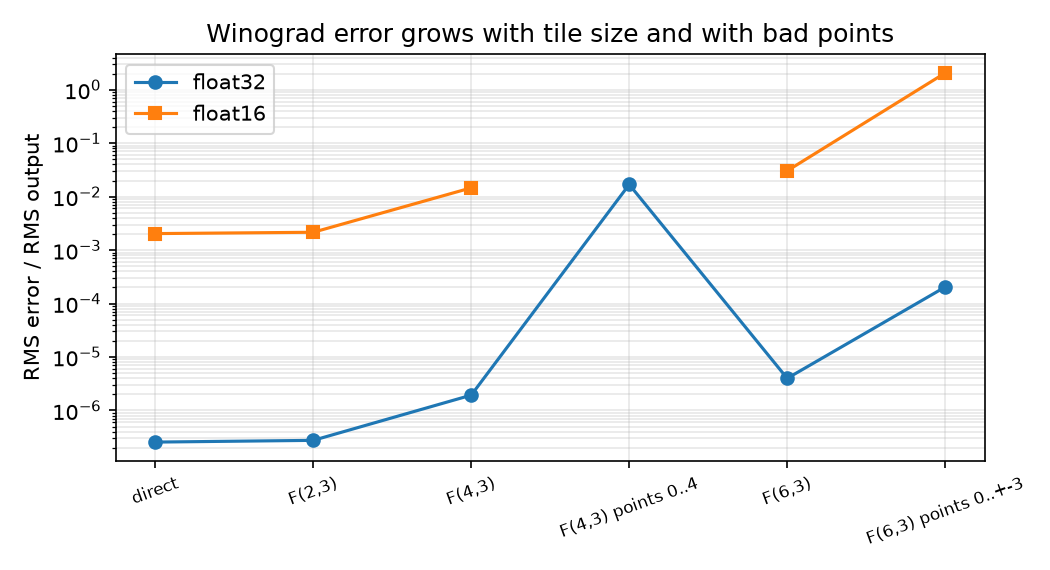
\includegraphics[width=0.85\linewidth]{winograd_numerics.png}
\caption{64 通道、$26\times26$ 输入、32 个输出通道的 3×3 卷积，相对 fp64 直接卷积的 rms 相对误差（对数纵轴）。蓝线 fp32，橙线 fp16；fp16 下“F(4,3) 点 0..4”溢出为 inf，图中没有点。}\label{fig:numerics}
\end{figure}

实验设置（\texttt{run\_experiments.py winograd\_numerics}）：输入取标准正态，权重按 $1/\sqrt{9C}$ 缩放，使输出量级约为 1；
用 NumPy 在指定 dtype 下完成所有变换、逐点乘与求和，与 fp64 直接卷积比较。

\begin{table}[H]
\centering\small
\caption{rms 相对误差（\texttt{winograd\_numerics.csv}）}\label{tab:numerics}
\begin{tabular}{lrrrr}
\toprule
变体 & 乘法减少 & 输入放大 & fp32 & fp16 \\
\midrule
direct & 1 & 1 & 2.6e-7 & 2.0e-3 \\
F(2,3) & 2.25 & 4 & 2.8e-7 & 2.2e-3 \\
F(4,3)，点 $\{0,\pm1,\pm2\}$ & 4 & 100 & 1.9e-6 & 1.5e-2 \\
F(6,3)，点 $\{0,\pm1,\pm2,\pm\tfrac12\}$ & 5.06 & 225 & 4.0e-6 & 3.0e-2 \\
F(4,3)，点 0..4 & 4 & 14,400 & 1.7e-2 & 溢出 \\
F(6,3)，点 $0..\pm3$ & 5.06 & 10,000 & 2.0e-4 & 2.06 \\
\bottomrule
\end{tabular}
\end{table}

\Cref{fig:numerics} 的两条线形状几乎平行，读法是：
\begin{itemize}
  \item \textbf{F(2,3) 免费}。fp32 下 2.8e-7 对直接卷积 2.6e-7（1.08 倍），fp16 下 2.2e-3 对 2.0e-3（1.06 倍），两条线在前两个点上几乎是平的。
  \item \textbf{好点集下误差随 tile 稳步增长}。F(4,3) 在 fp32 下是直接卷积的 7.6 倍、fp16 下 7.2 倍；F(6,3) 分别是 16 倍和 15 倍。
  fp32 下 4.0e-6 仍然完全可用；fp16 下 F(6,3) 的 rms 误差已经到 3\%。
  \item \textbf{点集选错是灾难}。图中间的尖峰是“F(4,3) 点 0..4”：同样少 4 倍乘法，输入放大从 100 变成 14,400，fp32 误差从 1.9e-6 跳到 1.7e-2（约 8700 倍），
  fp16 直接溢出。“F(6,3) 点 $0..\pm3$”的 fp32 误差是好点集的 51 倍，fp16 下 rms 误差 2.06，即误差比信号还大。
\end{itemize}
误差的排序与 \cref{tab:norms} 的输入放大基本一致，但不严格成比例：F(6,3) 点 $0..\pm3$ 的放大（10,000）低于 F(4,3) 点 0..4（14,400），fp32 误差却低两个数量级——
误差还取决于 $A^{\mathsf T}$、$G$ 的条件数与舍入在哪一步发生，放大只是一个上界。

\paragraph{为什么 C++ 的 F(2,3) 误差反而比 GEMM 小。} \texttt{conv\_bench.csv} 里，$56^2$ 层 Winograd 的相对误差是 4.0e-7，im2col / implicit 是 1.2e-6；
$14^2$ 层 5.9e-7 对 1.7e-6。GEMM 类实现每个输出要在 fp32 里顺序累加 $K = 9\cdot IC$ 项（576 或 2304 项），Winograd 的每个 GEMM 只累加 $IC$ 项（64 或 256），
再由输出变换合并 16 个部分和，累加链短了 9 倍；F(2,3) 的变换系数只有 $0,\pm1,\pm\tfrac12$，几乎不引入额外舍入。这和上面 NumPy 实验里“F(2,3) 与直接卷积同精度”是一致的。

\paragraph{int8。} F(2,3) 变换后的输入要 10 bit，F(4,3) 要 15 bit，逐点乘必须用 int16，吞吐减半，抵消一半乘法节省；
要么就在变换域重新量化，引入额外误差。这是 TFLite Micro、CMSIS-NN 不提供 int8 Winograd 的原因。

\begin{findingbox}[：精度决定能用多大的 tile]
fp32 上 F(4,3)、F(6,3) 都可用（误差 1.9e-6、4.0e-6）；fp16 上只有 F(2,3) 与直接卷积同精度，F(4,3) 已是 7.2 倍；int8 基本不用。
插值点必须用小而对称的点集：同样是 F(4,3)，点 0..4 在 fp16 下直接溢出。
\end{findingbox}

\section{本机与服务器对照}\label{sec:cross}

\begin{figure}[H]
\centering
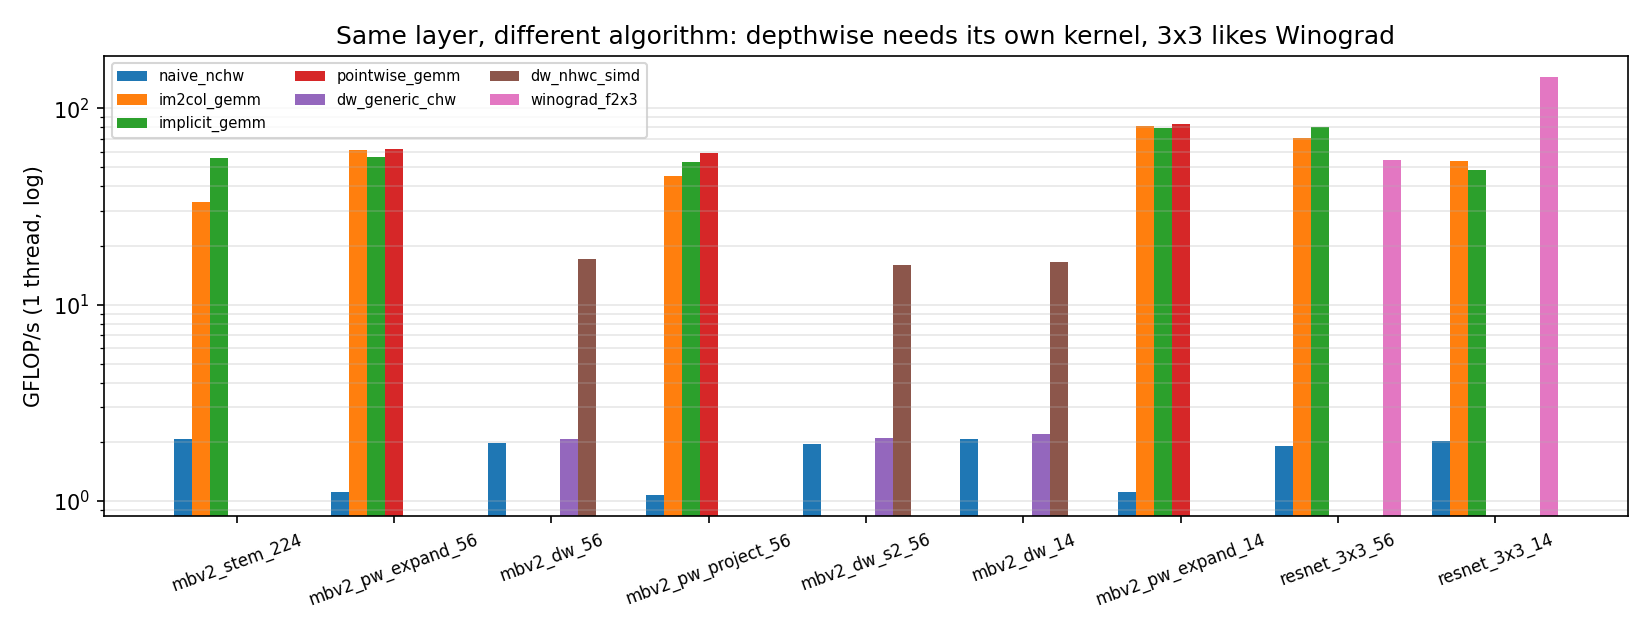
\includegraphics[width=\linewidth]{xeon8470q/conv_bench.png}
\caption{同一份代码在 Xeon Platinum 8470Q 上单线程的 GFLOP/s（对数纵轴，GCC 11.4，绑 NUMA1 物理核）。与 \cref{fig:bench} 对比：GEMM 类柱子整体上移一倍以上，$56^2$ 层的 Winograd（粉色）落到了 GEMM 柱子下方。}\label{fig:bench-xeon}
\end{figure}

\Cref{fig:bench-xeon} 与 \cref{fig:bench} 的整体形状相同，但有两处看得出来的变化：GEMM 类的橙、绿、红柱子从 15--37 升到 33--84 GFLOP/s；
\texttt{resnet\_3x3\_56} 一组里粉色的 Winograd 从“最高”变成“低于 im2col 和 implicit”，而 \texttt{resnet\_3x3\_14} 一组里它反而更突出（144.5，图中最高的柱子）。
depthwise 的棕色柱子只从约 11 升到约 16--17，与 GEMM 类拉开了距离。

\begin{table}[H]
\centering\small
\caption{服务器全部结果（GFLOP/s，\texttt{xeon8470q/conv\_bench.csv} 的 p50）}\label{tab:server}
\resizebox{\linewidth}{!}{\begin{tabular}{lrrrrrrr}
\toprule
层 & naive NCHW & im2col & implicit & pointwise & dw CHW & dw NHWC & Winograd \\
\midrule
\texttt{mbv2\_stem\_224} & 2.06 & 33.2 & \textbf{55.6} & & & & \\
\texttt{mbv2\_pw\_expand\_56} & 1.11 & 61.2 & 56.6 & \textbf{62.3} & & & \\
\texttt{mbv2\_dw\_56} & 1.98 & & & & 2.07 & \textbf{17.0} & \\
\texttt{mbv2\_pw\_project\_56} & 1.07 & 45.4 & 53.5 & \textbf{59.3} & & & \\
\texttt{mbv2\_dw\_s2\_56} & 1.94 & & & & 2.09 & \textbf{15.9} & \\
\texttt{mbv2\_dw\_14} & 2.07 & & & & 2.19 & \textbf{16.6} & \\
\texttt{mbv2\_pw\_expand\_14} & 1.11 & 81.6 & 79.1 & \textbf{83.6} & & & \\
\texttt{resnet\_3x3\_56} & 1.90 & 70.8 & \textbf{80.4} & & & & 54.3 \\
\texttt{resnet\_3x3\_14} & 2.02 & 54.1 & 48.2 & & & & \textbf{144.5} \\
\bottomrule
\end{tabular}}
\end{table}

服务器上的最大相对误差是 1.5e-6，小形状检查的误差与本机同一量级（最大 3.2e-7），两台机器上的 kernel 都是正确的。

\begin{table}[H]
\centering\small
\caption{服务器 / 本机的速度比，按实现分组}\label{tab:ratio}
\begin{tabular}{lrl}
\toprule
实现 & 服务器 / 本机 & 说明 \\
\midrule
GEMM 类（除 $14^2$ ResNet） & 1.99--2.81 & 高于 fp32 峰值之比 $232/154.9 = 1.50$ \\
im2col、implicit（$14^2$ ResNet） & 1.48、1.38 & 见下文 L2 的讨论 \\
Winograd F(2,3) & 1.37（$56^2$）、1.92（$14^2$） & \\
dw NHWC SIMD & 1.45--1.58 & 约等于峰值之比 \\
dw CHW 通用 & 1.64--1.73 & \\
naive NCHW & 1.61--2.27 & \\
\bottomrule
\end{tabular}
\end{table}

\paragraph{Winograd 的翻转。}

\begin{table}[H]
\centering\small
\caption{ResNet 3×3 层：本机 → 服务器（GFLOP/s）}\label{tab:flip}
\begin{tabular}{lrrr}
\toprule
层 & implicit GEMM & Winograd F(2,3) & Winograd / implicit \\
\midrule
$56^2$，64 → 64 & 34.3 → 80.4 & 39.7 → 54.3 & 1.16 → \textbf{0.68} \\
$14^2$，256 → 256 & 34.9 → 48.2 & 75.0 → 144.5 & 2.15 → 3.00 \\
\bottomrule
\end{tabular}
\end{table}

$56^2$ 层上 implicit GEMM 快了 2.34 倍，Winograd 只快 1.37 倍，于是 Winograd 从“快 16\%”变成“慢 32\%”。设 GEMM 部分时间为 $t_g$、变换时间为 $t_x$，
Winograd 相对 implicit GEMM 的收益约为
\begin{equation}
  S = \frac{t_g}{t_g/2.25 + t_x},\label{eq:flip}
\end{equation}
当 GEMM 变快、$t_x$ 不变时 $S$ 单调下降，$t_x > t_g(1-1/2.25)$ 时小于 1。\Cref{tab:tx} 的估计正是这种情形：$t_x$ 在两台机器上都是约 3 ms，$t_g$ 从 6.7 ms 降到 2.9 ms。
这是一个\emph{位置性}结论：它取决于 GEMM 速度与变换速度的相对大小，换机器就可能翻转。

\paragraph{$14^2$ 层为什么反而更划算。} 服务器上 $14^2$ 层的 implicit GEMM 只快了 1.38 倍，是所有 GEMM 类点里最少的，Winograd 对它的优势升到 3.00 倍，超过理论的 2.25。
按代码推算（没有计数器验证）：implicit GEMM 每个寄存器块只覆盖 4 个输出像素，要把整个 K 维的权重流一遍，$14^2$ 层的权重是 $2304\times256\times4\approx2.36$ MB，
超过本机每核 1.25 MiB 的 L2，每 4 个像素就从 L3 重读一次全部权重；而 Winograd 的每个 GEMM 只用一片 $256\times256\times4 = 262{,}144$ B 的 $U_e$，能留在 L2 里。
$56^2$ 层的权重只有 $576\times64\times4 = 147{,}456$ B，implicit GEMM 不受这个限制，所以它在服务器上能吃满更快的核（2.34 倍）。
同样的道理解释了 $14^2$ 层上 im2col 比 implicit 快（6 行寄存器块，每次读权重服务更多像素）：本机 1.05 倍，服务器 1.12 倍。

\paragraph{depthwise 的结构性结论。} NHWC SIMD 对 CHW 通用实现：本机 8.2--9.0 倍，服务器 7.6--8.2 倍（$56^2$ 层 8.2 倍）。
depthwise NHWC 只快 1.45--1.58 倍，与单核 fp32 峰值之比 1.50 相当，低于 GEMM 类的 2--2.8 倍；所以倒残差块里 depthwise 的时间占比从 33.4\% 升到 40.1\%（\cref{tab:block}）。
服务器上 stride 2 层的 15.9 GFLOP/s 超过了按 0.9 FLOP/B × 17.5 GB/s 算出的 DRAM 屋顶（15.75），再次说明计时时数据在缓存里，这一列不能当带宽受限的证据。

\paragraph{im2col 的拷贝同样是“非 GEMM”开销。} 本机 $56^2$ ResNet 层上 im2col 与 implicit 几乎相同（33.9 对 34.3），服务器上 im2col 慢 12\%（70.8 对 80.4）；
1×1 project 层上 pointwise 对 im2col 的优势从 19\% 扩大到 31\%。7.2 MB / 1.8 MB 的展开拷贝和 Winograd 的变换一样，不随 FMA 吞吐变快。

\begin{figure}[H]
\centering
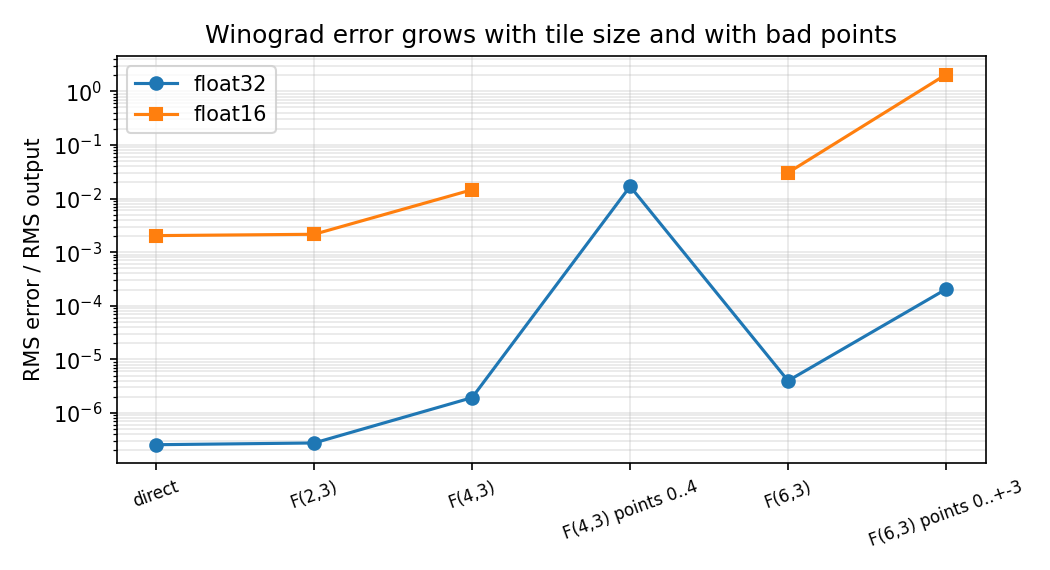
\includegraphics[width=0.85\linewidth]{xeon8470q/winograd_numerics.png}
\caption{服务器上重跑的 Winograd 数值实验。与 \cref{fig:numerics} 逐点相同。}\label{fig:numerics-xeon}
\end{figure}

\Cref{fig:numerics-xeon} 与 \cref{fig:numerics} 完全一致：两台机器的 \texttt{summary.json} 里 12 个 \texttt{wino\_rms\_*} 值逐位相同。
数值实验是固定随机种子（\texttt{default\_rng(0)}）的 NumPy 计算，fp32 / fp16 的 IEEE 舍入与 CPU 型号无关，这张图在服务器上只起“流水线可复现”的作用，不提供新信息。

\begin{findingbox}[：哪些结论跟着机器走]
\textbf{结构性}（换机器只改常数）：im2col 工作区（由 E19 决定）、depthwise 的 NHWC 优势（8.2 倍上下）、Winograd 的数值误差（逐位相同）。
\textbf{位置性}（可能翻转）：Winograd 是否比 GEMM 快——取决于 GEMM 有多快和变换域数据放不放得进缓存；im2col 与 implicit 谁快——取决于拷贝和寄存器块的相对代价。
\end{findingbox}

\section{面试追问}\label{sec:iq}

\begin{iqbox}{给你一个 3×3 卷积，你会怎么实现？}
先看数据类型与目标。MCU 上 int8：partial im2col（一次 2 个输出位置）加 GEMM 微核，或 implicit GEMM；完整 im2col 的工作区（E19）在 ResNet $56^2\times64$ 上是 7.2 MB fp32、int8 也要 1.8 MB，放不下。
CPU fp32：implicit GEMM 打底（本机与 im2col 最多相差 1.15 倍，工作区 0）；通道多、空间小、stride 1 时考虑 Winograd F(2,3)（$14^2\times256$ 上 2.15 倍）；
但要在目标机器上实测，因为同一层 $56^2\times64$ 在 Ice Lake 上快 16\%、在 Sapphire Rapids 上慢 32\%。depthwise 单独写 NHWC 的 SIMD kernel，1×1 直接当 GEMM。
\end{iqbox}

\begin{iqbox}{depthwise 参数和计算量都很少，为什么它慢？}
参数少只说明权重流量小，激活流量还在。fp32 3×3 的强度只有 4.5 FLOP/B（E21），按输入、输出各一次算是 2.25，没有 K 维可以做寄存器分块，GEMM 化无济于事。
本机同一个 $56^2$ 倒残差块里 depthwise 占 MACs 的 15.8\%、占时间的 33.4\%（服务器 40.1\%）。救法是布局：NHWC 让通道维连续，一条 512 位指令算 16 个通道，
比按通道的 CHW 实现快 8.2--9.0 倍；再进一步是与相邻 1×1 融合，让 depthwise 的输入不落回内存。
\end{iqbox}

\begin{iqbox}{Winograd 乘法少 2.25 倍，为什么实测只有 1.16 倍？换台更快的机器会更好吗？}
理论值只数逐点乘。变换的运算量 $\propto T(IC+OC)$，逐点乘 $\propto T\cdot IC\cdot OC$，相对开销约 $2/C$：$C = 64$ 是 $C = 256$ 的 4 倍；
而且变换是标量、逐 tile 的散布读写，$56^2$ 层的变换域缓冲 6.4 MB 超出 L2。按“GEMM 部分与 implicit GEMM 同速”估计，变换占了一半时间。
换更快的机器不一定更好：Xeon 8470Q 上 GEMM 快了 2.34 倍、变换几乎不变（估计 2.84 → 2.98 ms），Winograd 反而比 implicit GEMM 慢 32\%。
所以 cuDNN、ARM Compute Library 这类库在运行时按层、按设备测量后选算法，而不是写死。
\end{iqbox}

\begin{iqbox}{fp16 / int8 部署能用 Winograd 吗？用多大的 tile？}
fp16 只用 F(2,3)：误差 2.2e-3，与直接卷积的 2.0e-3 相同；F(4,3) 是 7.2 倍（1.5e-2），F(6,3) 到 3\%。输入放大 $\|B^{\mathsf T}\|_\infty^2$ 在 F(4,3) 是 100，约吃掉 6.6 bit，fp16 只有 11 位尾数。
插值点不能乱选：F(4,3) 换成点 0..4 时放大 14,400 倍，fp16 直接溢出。int8 输入经 F(2,3) 变换后最大 508（10 bit），F(4,3) 要 15 bit，逐点乘必须 int16，吞吐减半，
节省被抵消一半，还要处理变换域的重新量化，所以 TFLite Micro、CMSIS-NN 不提供 int8 Winograd。
\end{iqbox}

\begin{iqbox}{implicit GEMM 的代价是什么？为什么在 stem 上反而比 im2col 快？}
代价是 A 矩阵地址不连续：每 $IC$ 个元素要按 $(k_h,k_w)$ 重新算源地址、判断 padding（本 lab 用“越界指向全零行”消掉内层分支）。
$IC$ 小的时候这个开销似乎更大，但 im2col 在同样的位置要做一次 \texttt{memcpy}：stem 上每次只拷 3 个 float，一共 112,896 次，而 GEMM 的 K 维只有 27。
所以 stem 上 implicit GEMM 快 1.76 倍（服务器 1.68 倍）。GPU 上 implicit GEMM 的地址计算由硬件地址生成或 TMA 隐藏，CPU 上可以预计算偏移表。
\end{iqbox}

\section{结论}\label{sec:conclusion}

\begin{findingbox}[：五条可以带走的结论]
\begin{enumerate}[label=(\arabic*)]
  \item implicit GEMM 与 im2col 的算术相同、累加顺序相同、误差逐位相同，速度最多相差 1.15 倍（stem 除外，implicit 快 1.8 倍），工作区从最多 7.2 MB 降到 0。
  \item 1×1 卷积直接当 GEMM，省掉的拷贝越大越划算：$56^2$ 两层快 7--19\%（服务器 2--31\%），$14^2$ 层持平。
  \item depthwise 的速度由布局决定：NHWC + SIMD 比 CHW 快 8.2--9.0 倍；它占倒残差块 15.8\% 的 MACs、33.4\%--40.1\% 的时间。
  \item Winograd F(2,3) 的收益由变换占比决定：$14^2\times256$ 上 2.15 倍、$56^2\times64$ 上 1.16 倍；GEMM 变快后后者翻转为 0.68 倍。
  \item Winograd 的误差由变换矩阵的范数决定：fp16 只有 F(2,3) 与直接卷积同精度，F(4,3) 7.2 倍，坏点集直接溢出；int8 需要 10--15 bit。
\end{enumerate}
\end{findingbox}

\section{20 秒讲法}\label{sec:pitch}

我在 9 个 MobileNetV2 和 ResNet 层上用 C++ 写了 7 种 fp32 卷积 kernel，都对 fp64 参考验证过。implicit GEMM 和 im2col 一样快，但不要工作区，
im2col 在 ResNet $56^2$ 层上要 7.2 MB，是激活的 4.5 倍。depthwise 换成 NHWC 加 AVX-512 快 9 倍，可它只占 16\% 的计算、却占三分之一的时间。
Winograd F(2,3) 在通道多的层上快 2.15 倍，通道少的层上只有 1.16 倍；换到 Sapphire Rapids 上 GEMM 快了一倍，同一层 Winograd 反而慢 32\%。
数值上 fp16 只能用 F(2,3)，F(4,3) 误差是 7 倍，点选错直接溢出。

\begin{caveatbox}
\begin{itemize}
  \item 不能推出 Winograd 在别的 CPU 上的加速：它依赖 L2 容量与通道数，本机 $56^2$ 层的 1.16 倍和 $14^2$ 层的 2.15 倍差了一倍，换到 Xeon 8470Q 上前者变成 0.68 倍。
  \item “depthwise 占时间 33.4\%”是这个实现下的比例；1×1 再优化（打包、寄存器分块）后，depthwise 的占比只会更高。
  \item 全部是单线程结果；多线程下 depthwise 会先撞上带宽屋顶，各实现的相对排序可能改变。
  \item 这是 fp32 的 x86 kernel，TinyEngine 是 int8 的 MCU kernel：讲的是同样的布局与工作区问题，速度数字不能搬到 Cortex-M。
  \item 教学 GEMM 没有 B 打包和调过的寄存器分块，只到 fp32 峰值的 10--24\%；生产库里 GEMM 更快，按 \cref{eq:flip}，Winograd 与 im2col 的相对收益会更小。
  \item 只实现了 F(2,3) 的 C++ kernel；F(4,3)、F(6,3) 只做了数值实验，没有速度数字。
  \item 计时时同一份数据被反复调用、留在缓存里，表中“占 DRAM 屋顶”的比例不是带宽受限的证据；变换时间（\cref{tab:tx}）与 L2 的解释是由 p50 和代码推算的，没有硬件计数器验证。
\end{itemize}
\end{caveatbox}

\section{复现}\label{sec:repro}

\begin{lstlisting}[language=bash]
cd solutions/edge-runtime/conv-kernels
python -m pytest -q tests                           # Toom-Cook construction, 1-D/2-D exactness, all C++ kernels vs fp64
python scripts/run_experiments.py --only winograd   # numerics, seconds
python scripts/run_experiments.py --only bench      # timing, ~25 s, idle machine, 1 thread
\end{lstlisting}

\texttt{bench} 一步做三件事：
\begin{itemize}
  \item 用 \nolinkurl{edge_harness/cpp.py} 编译 \nolinkurl{cpp/conv.cpp}，\\选项为 \texttt{-O3 -std=c++17 -march=native -fno-math-errno}；
  \item 跑 \texttt{--mode=check}，写出 \nolinkurl{artifacts/raw/cpp_check.csv}；
  \item 跑 \texttt{--mode=bench --layer=all --repeats=15}，写出 \nolinkurl{conv_bench.jsonl} 与 \nolinkurl{conv_bench.csv}。
\end{itemize}
两步结束后都会重新生成 \nolinkurl{summary.json}，图在 \nolinkurl{artifacts/figures/}。服务器结果在 \nolinkurl{artifacts/raw/xeon8470q/}
与 \nolinkurl{artifacts/figures/xeon8470q/}，是同一命令在绑核（\texttt{taskset}，NUMA1 物理核）的容器里运行的输出。
跨主机的汇总见仓库的 \nolinkurl{interview/CROSS-HOST.md}。


\begin{thebibliography}{99}
\bibitem{chellapilla2006} K.~Chellapilla, S.~Puri, P.~Simard. High Performance Convolutional Neural Networks for Document Processing. \emph{IWFHR}, 2006.
\bibitem{lavin2016} A.~Lavin, S.~Gray. Fast Algorithms for Convolutional Neural Networks. \emph{CVPR}, 2016.
\bibitem{mobilenetv2} M.~Sandler, A.~Howard, M.~Zhu, A.~Zhmoginov, L.-C.~Chen. MobileNetV2: Inverted Residuals and Linear Bottlenecks. \emph{CVPR}, 2018.
\bibitem{resnet} K.~He, X.~Zhang, S.~Ren, J.~Sun. Deep Residual Learning for Image Recognition. \emph{CVPR}, 2016.
\bibitem{mcunet} J.~Lin, W.-M.~Chen, Y.~Lin, J.~Cohn, C.~Gan, S.~Han. MCUNet: Tiny Deep Learning on IoT Devices. \emph{NeurIPS}, 2020.
\end{thebibliography}

\end{document}
